\documentclass{beamer}
\usepackage{lmodern}
\usepackage[T1]{fontenc}
\usepackage[utf8]{inputenc}
\usepackage[magyar]{babel}
\usepackage{standalone}
\usepackage{adjustbox}
\usepackage{tikz}

\usetikzlibrary{shapes, positioning, mindmap, arrows.meta}
\newcommand{\tikzmark}[1]{\tikz[overlay,remember picture] \node (#1) {};}

% straight from http://tex.stackexchange.com/a/55849/8785
  \tikzset{
    invisible/.style={opacity=0},
    visible on/.style={alt={#1{}{invisible}}},
    alt/.code args={<#1>#2#3}{%
      \alt<#1>{\pgfkeysalso{#2}}{\pgfkeysalso{#3}} % \pgfkeysalso doesn't change the path
    },
  }
\title{A PLanG programozási nyelv kiterjesztése}
\subtitle{Önálló laboratóriumi beszámoló}
\author{Scipiades Ármin\\\bigskip Konzulens: Dr.\thinspace Feldhoffer Gergely}
\date{2015. május 27.}

\usetheme{Rochester}
\usecolortheme{beaver}
\setbeamertemplate{navigation symbols}{}

\begin{document}

\frame{\titlepage}

\begin{frame}
	\frametitle{A PLanG programozási nyelv}
	\centering
	\includegraphics[width=\linewidth,height=\textheight,keepaspectratio]{images/plang.pdf}
\end{frame}

\begin{frame}
	\frametitle{A programozási nyelv felhasználói felület}	
	\centering
	\begin{adjustbox}{max totalsize={\textwidth}{\textheight},center}
	\begin{tikzpicture}[
	node distance=10cm,
	stuff/.style={draw, cloud, cloud ignores aspect, font=\Huge},
	img/.style={text width=3cm, minimum height=3cm},
	arr/.style={->, >={Latex[length=0.4cm]}, shorten >=1pt},
	label/.style={fill=white, font=\Huge}
]

\node[stuff] (input) {Feladat};
\node[img, below= 3cm of input] (human) {{\includestandalone[width=\textwidth]{images/human_head}}};
\node[img, right of=human, text width=6cm] (language) {{\includegraphics[width=\textwidth]{images/plang.pdf}}};
\node[img, right of=language] (computer) {{\includestandalone[width=\textwidth]{images/computer}}};
\node[stuff, above=3cm of computer] (output) {Megoldás};

\draw[arr] (input) edge (human);
\draw[arr] (human) edge node[label] {algoritmus} (language);
\draw[arr] (language) edge node[label] {program} (computer);
\draw[arr] (computer) edge (output);

\end{tikzpicture}

	\end{adjustbox}	
\end{frame}

\begin{frame}
	\frametitle{Programozási nyelvek minőségi mutatói}
	\centering
	\begin{adjustbox}{max totalsize={\textwidth}{\textheight},center}
	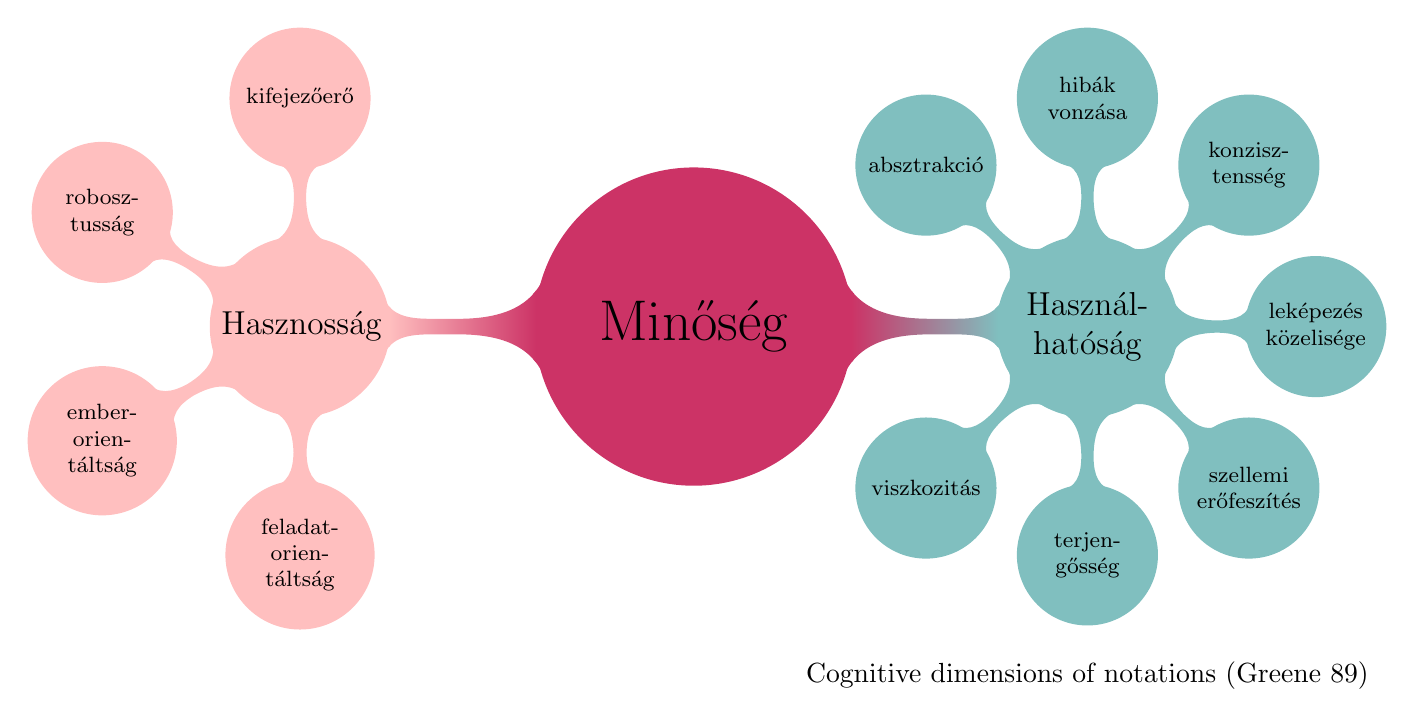
\begin{tikzpicture}
	\path[
		mindmap,
		concept color=purple!80,
		text=black
	]
		node [concept, font=\huge] {Minőség}
		[clockwise from=0, level 1 concept/.append style={sibling angle=180}]
		child[concept color=teal!50] {
			node[concept, font=\large] (usability) {Hasz\-nál\-ha\-tó\-ság}
			[clockwise from=135, level 2 concept/.append style={sibling angle=45, visible on=<3->}]
			child { node[concept] {absztrakció} }
			child { node[concept] {hibák vonzása} }
			child { node[concept] {kon\-zisz\-tens\-ség} }
			child { node[concept] {leképezés közelisége} }
			child { node[concept] {szellemi erőfeszítés} }
			child { node[concept] {ter\-jen\-gős\-ség} }
			child { node[concept] {viszkozitás} }
		}
		child[concept color=pink] {
			node[concept, font=\large] {Hasznosság}
			[counterclockwise from=90, level 2 concept/.append style={sibling angle=60, visible on=<2->}]
			child { node[concept] {ki\-fe\-je\-ző\-e\-rő} }
			child { node[concept] {ro\-bosz\-tus\-ság} }
			child { node[concept] {ember\-orien\-táltság} }
			child { node[concept] {feladat\-orien\-táltság} }
		};

		\node[below=3 of usability, visible on=<3->] {Cognitive dimensions of notations (Greene 89)};
\end{tikzpicture}

	\end{adjustbox}
\end{frame}


\end{document}